%%%%%%%%%%%%%%%%%%%%%%%%%%%%%%%%%%%%
% Slide options
%%%%%%%%%%%%%%%%%%%%%%%%%%%%%%%%%%%%

% Option 1: Slides with solutions

\documentclass[slidestop,compress,mathserif]{beamer}
\newcommand{\soln}[1]{\textit{#1}}
\newcommand{\solnGr}[1]{#1}

% Option 2: Handouts without solutions

% \documentclass[11pt,containsverbatim,handout]{beamer}
% \usepackage{pgfpages}
% \pgfpagesuselayout{resize to}[letterpaper,landscape,border shrink=5mm]
% \newcommand{\soln}[1]{ }
% \newcommand{\solnGr}{ }

%%%%%%%%%%%%%%%%%%%%%%%%%%%%%%%%%%%%
% Style
%%%%%%%%%%%%%%%%%%%%%%%%%%%%%%%%%%%%

\def\chp9@path{../../../Chp 9}
\input{../../lec_style.tex}

%%%%%%%%%%%%%%%%%%%%%%%%%%%%%%%%%%%%
% Preamble
%%%%%%%%%%%%%%%%%%%%%%%%%%%%%%%%%%%%

\title[Lecture 36]{MA213: Lecture 36}
\subtitle{Module 5: Beyond Recipes: Frequentist and Bayesian Approaches to Statistical Modeling}
\author{OpenIntro Statistics, 4th Edition}
\institute{$\:$ \\ {\footnotesize Based on slides developed by Mine \c{C}etinkaya-Rundel of OpenIntro. \\
The slides may be copied, edited, and/or shared via the \webLink{http://creativecommons.org/licenses/by-sa/3.0/us/}{CC BY-SA license.} \\
Some images may be included under fair use guidelines (educational purposes).}}
\date{}


%%%%%%%%%%%%%%%%%%%%%%%%%%%%%%%%%%%%
% Begin document
%%%%%%%%%%%%%%%%%%%%%%%%%%%%%%%%%%%%

\begin{document}


%%%%%%%%%%%%%%%%%%%%%%%%%%%%%%%%%%%%
% Title page
%%%%%%%%%%%%%%%%%%%%%%%%%%%%%%%%%%%%

{
\addtocounter{framenumber}{-1} 
{\removepagenumbers 
\usebackgroundtemplate{
\includegraphics[width=\paperwidth]{../../OpenIntro_Grid_4_3-01.jpg}}
\begin{frame}

\hfill 
\includegraphics[width=20mm]{../../oiLogo_highres}

\titlepage

\end{frame}
}
}


%%%%%%%%%%%%%%%%%%%%%%%%%%%%%%%%%%%%
% Recap/Agenda
%%%%%%%%%%%%%%%%%%%%%%%%%%%%%%%%%%%%
% TODO better formatting
\begin{frame}
    \frametitle{Module 5: Beyond Recipes: Frequentist and Bayesian Approaches to Statistical Modeling}
    \begin{itemize}
        \item \hl{Previously: }Case study in modern statistical modeling
        \item \hl{This time: }Wrap-up and evaluations
        \item \hl{Reading: }(none)
    \end{itemize}

\end{frame}


%%%%%%%%%%%%%%%%%%%%%%%%%%%%%%%%%%%%
% Deadlines/Announcements
%%%%%%%%%%%%%%%%%%%%%%%%%%%%%%%%%%%%
\begin{frame}
    \frametitle{Deadlines/Announcements}
\begin{itemize}
            \item Quiz 5 Almost Pass Office Hours are Thursday and Friday this week
            \item Final Exam Block Quiz retake choice form due Friday December 12 at 11:59pm
            \item Final Exam Block is Monday December 15, 1:00pm-2:00pm in PHO 206 (our usual room)
        \end{itemize}
\end{frame}

%%%%%%%%%%%%%%%%%%%%%%%%%%%%%%%%%%%%
% Sections
%%%%%%%%%%%%%%%%%%%%%%%%%%%%%%%%%%%%

\section{Evaluations}

%%%%%%%%%%%%%%%%%%%%%%%%%%%%%%%%%%%%

\begin{frame}
\frametitle{Your feedback is very important to us!}
Please take 15 minutes to complete (if you haven't already):
\begin{itemize}
    \item Course Evaluation A1 
    \begin{itemize}
        \item Lecture/Overall
        \item Accessed through the course website on Blackboard
    \end{itemize}
    \item The LCT survey
    \begin{itemize}
        \item Used for deciding what to keep/change for next time and evaluating the effectiveness of the Course Transformation
        \item Accessed through the link sent to your BU email, titled ``Extra Credit Survey Link, MA213 Basic Statistics and Probability (Fall 2025)''
    \end{itemize}
\end{itemize}
\end{frame}

%%%%%%%%%%%%%%%%%%%%%%%%%%%%%%%%%%%%

\begin{frame}
\frametitle{Extra Credit Survey Link, MA213 Basic Statistics and Probability (Fall 2025)}
% The survey_email.png asset is not currently tracked in the repository.
\end{frame}


%%%%%%%%%%%%%%%%%%%%%%%%%%%%%%%%%%%%

\section{Quiz 5 Solutions}

%%%%%%%%%%%%%%%%%%%%%%%%%%%%%%%%%%%%

\section{Wrap up}

%%%%%%%%%%%%%%%%%%%%%%%%%%%%%%%%%%%
% Big picture of statistics 
% https://stats.libretexts.org/Bookshelves/Applied_Statistics/Biostatistics_-_Open_Learning_Textbook/Preliminaries/The_Big_Picture
% https://creativecommons.org/licenses/by-nc-sa/4.0/

\begin{frame}
    \frametitle{Big Picture of Statistics}
    \begin{center}
        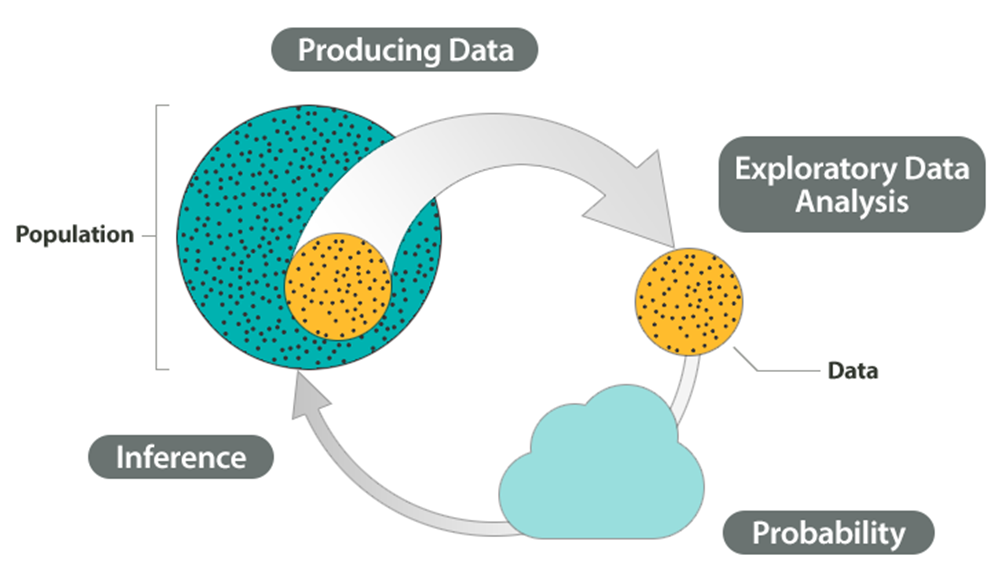
\includegraphics[width=0.95\textwidth]{../../Module1/lecture1/figures/BigPicture1.png}
    \end{center}
    \vspace{0.5em}
    \footnotesize
    Credit: \href{https://stats.libretexts.org/Bookshelves/Applied_Statistics/Biostatistics_-_Open_Learning_Textbook/Preliminaries/The_Big_Picture}{LibreTexts}
    \\
    Licensed under \href{https://creativecommons.org/licenses/by-nc-sa/4.0/}{CC BY-NC-SA 4.0}
\end{frame}

\begin{frame}
    \frametitle{Big Picture of Statistics}
    \begin{center}
        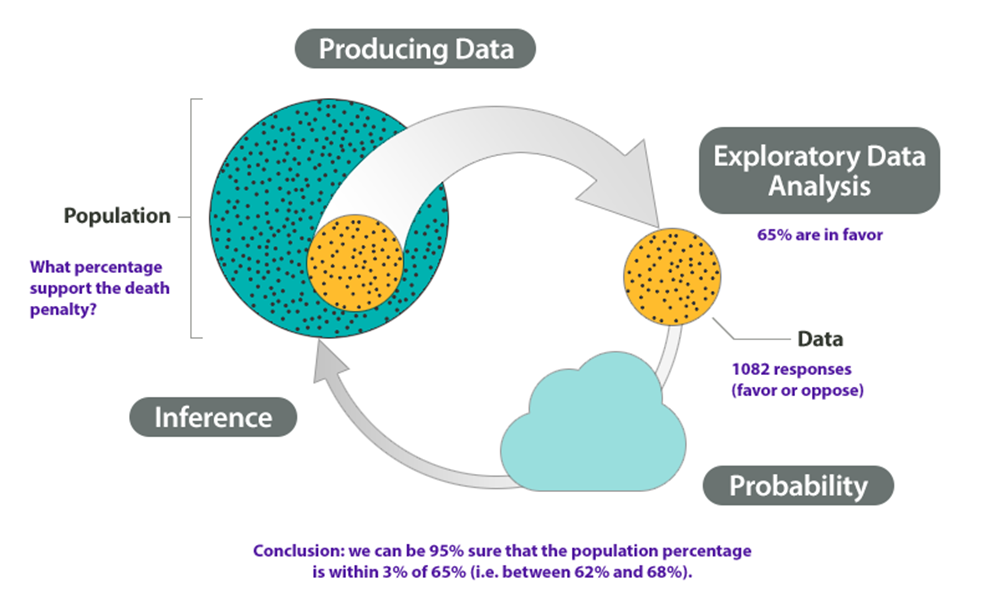
\includegraphics[width=0.95\textwidth]{../../Module1/lecture1/figures/BigPicture2.png}
    \end{center}
    \vspace{0.5em}
    \footnotesize
    Credit: \href{https://stats.libretexts.org/Bookshelves/Applied_Statistics/Biostatistics_-_Open_Learning_Textbook/Preliminaries/The_Big_Picture}{LibreTexts}
    \\
    Licensed under \href{https://creativecommons.org/licenses/by-nc-sa/4.0/}{CC BY-NC-SA 4.0}
\end{frame}

%%%%%%%%%%%%%%%%%%%%%%%%%%%%%%%%%%%%

\begin{frame}
\frametitle{The course modules take us through the big picture}
\begin{itemize}
\item Module 1: Exploratory Data Analysis and Study Design
\item Module 2: Probability, Random Variables, and Distributions 
\item Module 3: Foundations for Inference
\item Module 4: Inference
\item Module 5: Linear Regression
\end{itemize}

\end{frame}

%%%%%%%%%%%%%%%%%%%%%%%%%%%%

\begin{frame}
\frametitle{It all comes down to modeling}
\begin{center}
    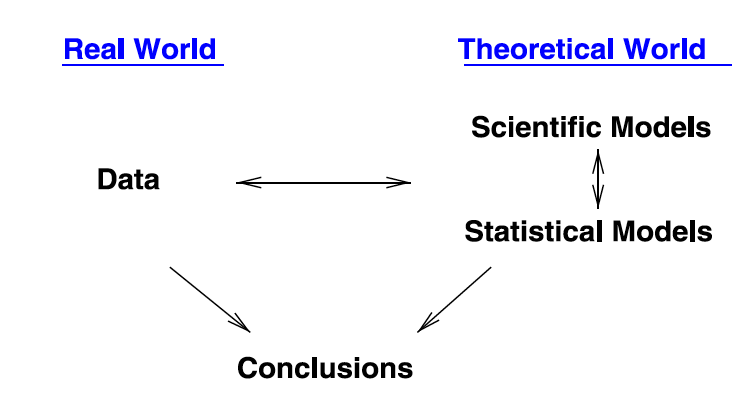
\includegraphics[width=0.8\textwidth]{Kass2011_1.png}
\end{center}
\footnotesize{Kass, R. E. (2011). Statistical inference: The big picture. \textit{Statistical Science}, 26(1), 1-9. \url{https://doi.org/10.1214/10-STS337}}
\end{frame}

\begin{frame}
\frametitle{It all comes down to modeling... which can get complicated!}
\begin{center}
    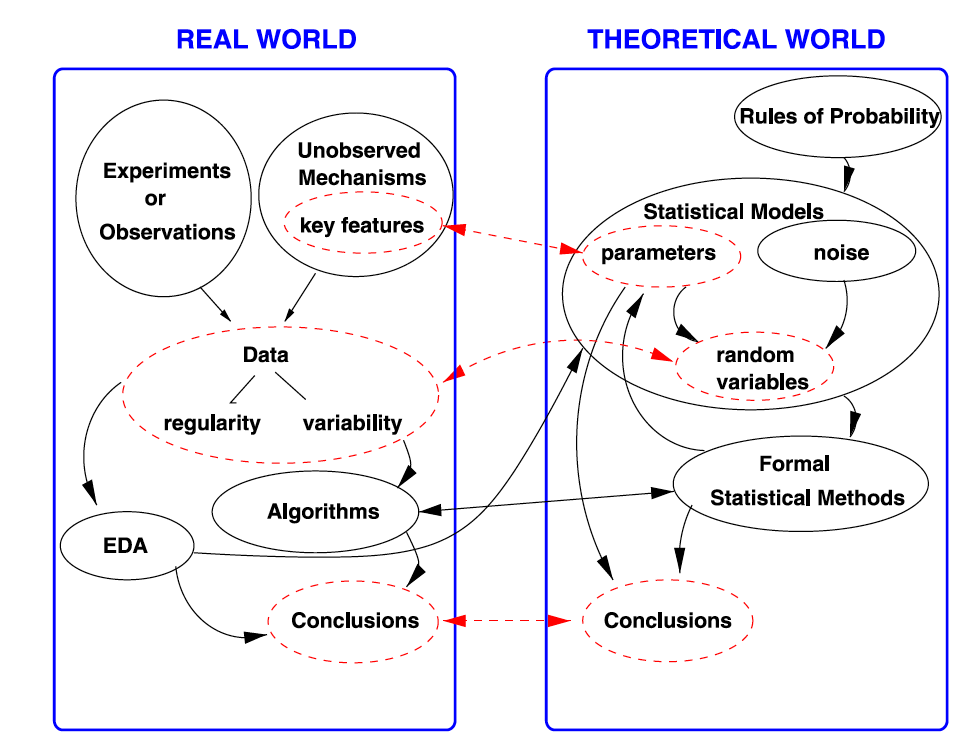
\includegraphics[width=0.8\textwidth]{Kass2011_2.png}
\end{center}
\footnotesize{Kass, R. E. (2011). Statistical inference: The big picture. \textit{Statistical Science}, 26(1), 1-9. \url{https://doi.org/10.1214/10-STS337}}
\end{frame}

\begin{frame}
\frametitle{In practice, statistical modeling is iterative (Box/Tukey)}
\begin{center}
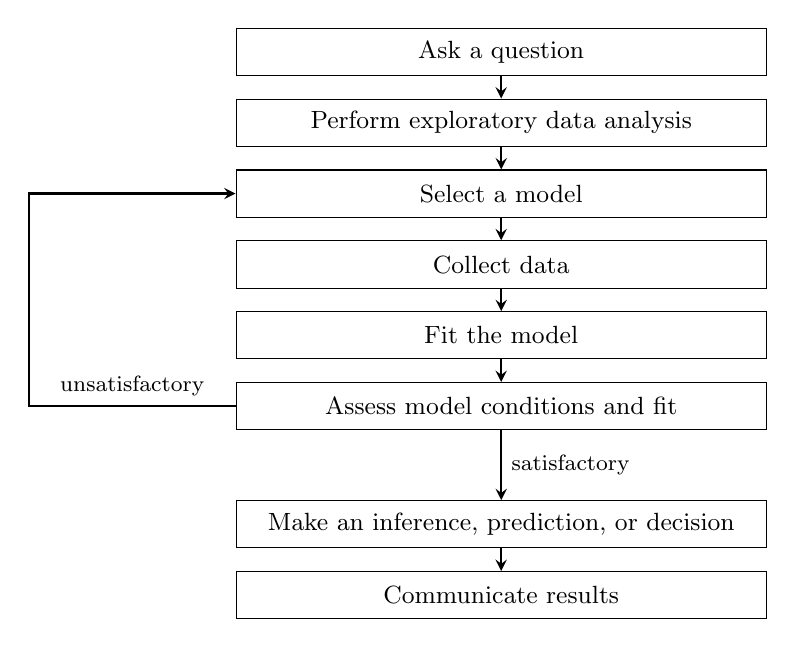
\begin{tikzpicture}[
    node distance=0.9cm,
    box/.style={rectangle, draw, text width=6.5cm, align=center, minimum height=0.6cm, font=\small},
    arrow/.style={->, >=stealth, thick}
]

% Nodes
\node[box] (q1) {Ask a question};
\node[box, below of=q1] (q2) {Perform exploratory data analysis};
\node[box, below of=q2] (q3) {Select a model};
\node[box, below of=q3] (q4) {Collect data};
\node[box, below of=q4] (q5) {Fit the model};
\node[box, below of=q5] (q6) {Assess model conditions and fit};
\node[box, below of=q6, node distance=1.5cm] (q7) {Make an inference, prediction, or decision};
\node[box, below of=q7] (q8) {Communicate results};

% Arrows
\draw[arrow] (q1) -- (q2);
\draw[arrow] (q2) -- (q3);
\draw[arrow] (q3) -- (q4);
\draw[arrow] (q4) -- (q5);
\draw[arrow] (q5) -- (q6);
\draw[arrow] (q6) -- node[right, font=\footnotesize] {satisfactory} (q7);
\draw[arrow] (q7) -- (q8);
\draw[arrow] (q6) -- node[above, font=\footnotesize] {unsatisfactory} ++(-6,0) |- (q3);

\end{tikzpicture}
\end{center}
\end{frame}

%%%%%%%%%%%%%%%%%%%%%%%%%%%%

\begin{frame}
\frametitle{Models can be wrong, but useful}

\begin{quote}
All models are wrong, but some are useful. - George Box
\end{quote}

\begin{itemize}

\item No model is perfect, but even imperfect models can be useful, as long as we are clear and report the model's shortcomings.

\item If conditions are grossly violated, we should not report the model results, but instead consider a new model, even if it means learning more statistical methods or hiring someone who can help.

\end{itemize}

\end{frame}

%%%%%%%%%%%%%%%%%%%%%%%%%%%%

\begin{frame}
    \frametitle{Thank you!}

    What we learned in this class is the foundation for:
    \begin{itemize}
        \item Data science, ML, and AI (including genAI)
        \item Brain-computer interfaces
        \item Public health
        \item Genetics
        \item Quantitative Finance
        \item Quantum physics / quantum computing
        \item etc etc etc
    \end{itemize}

    I hope you enjoyed the course and continue exploring statistics in the future!

\end{frame}
%%%%%%%%%%%%%%%%%%%%%%%%%%%%%%%%%%%%

%%%%%%%%%%%%%%%%%%%%%%%%%%%%%%%%%%%%
% End document
%%%%%%%%%%%%%%%%%%%%%%%%%%%%%%%%%%%%

\end{document}
